\subsection{Electrical Power System}

\paragraph{}The electric power system of the satellite must provide and manage the energy generated efficiently in order to have all the systems operating under normal conditions during the lifetime of the mission. The EPS of the Cubesat is, probably, the most fundamental requirement of the satellite, since its failure would result in a mission failure. 

\paragraph{}The energy collection system and the power management and  collection systems compose the EPS and their role is to control and distribute power to the Cubesat, to suppy a continuous source of electrical power during the length of the mission, to protect the satellite against electrical bus failiures and to monitor and communicate the status of the EPS to the on-board computer.

\begin{figure}[h]
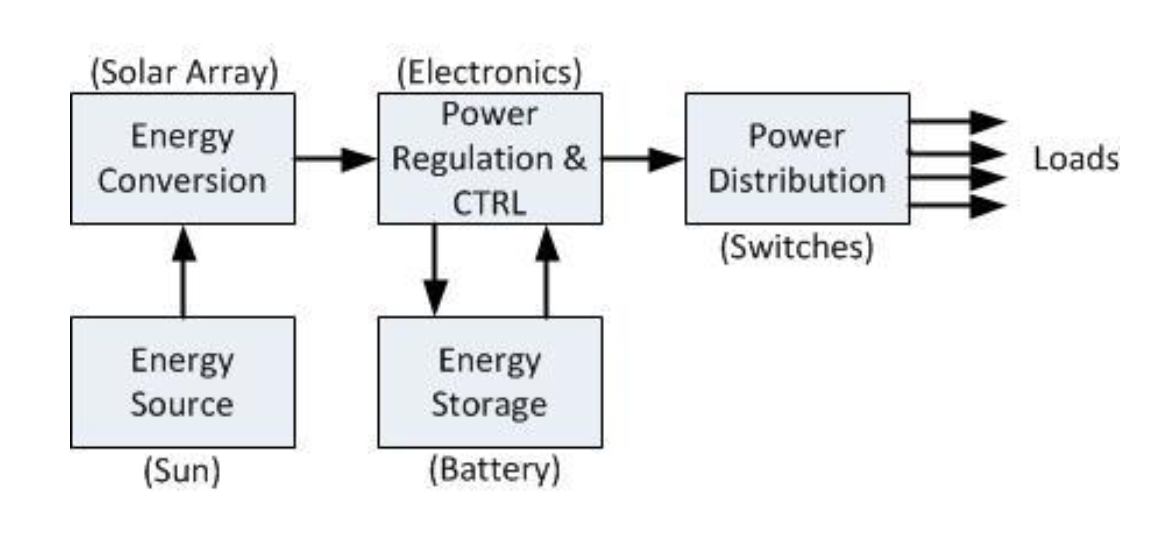
\includegraphics[scale=0.6]{./sections/SatelliteDesign/images/epsbasics}
\centering
\caption{Basic schematics of the EPS} 
\cite{epsbasics}
\end{figure}

\subsubsection{Estimation of the power required}
\paragraph{}To select the adequate electrical power systems it is essential that the power consumed by the CubeSat is known \textit{a priori}. Thus, to select the solar arrays and the batteries, as well as the power management system, an estimation of the power consumed has to be made.

\paragraph{}The vast majority of the time the satellite will work under typical operation conditions. However, the estimation of the power consumption provided in the table \ref{powerestimation} has been made for typical-high conditions in order to have a power margin and a more reliable estimation.


\begin{longtable}{| l | r | }
\hline
\rowcolor[gray]{0.80}	\textbf{System (number of units)} &  \textbf{Typical power consumption per unit (W)} \\
\hline
\endfirsthead

\rowcolor[gray]{0.85} \textbf{Payload} &  \\
	   ~Patch antenna (8) & 4 \\
	   \rowcolor[gray]{0.95} \textbf{Payload power consumption} & 32 \\
	   \hline
	\hline

\rowcolor[gray]{0.85} \textbf{Electrical Power System} &  \\
	   ~NanoPower P60 Power Module (1) & 2 \\
	   ~Battery (2) & - \\
	   ~Solar arrays (4) & -\\
	   \rowcolor[gray]{0.95} \textbf{EPS power consumption} & 2 \\
	   \hline
	\hline
	
\rowcolor[gray]{0.85} \textbf{Data Handling Systems} &  \\
	   ~Transceiver inner-satellite (3) & 4 \\
	   ~Transceiver space to ground (1) & 4 \\
	   ~Data handling system (1) & 4 \\
	   \rowcolor[gray]{0.95} \textbf{DHS power consumption} & 15 \\
	   \hline
	\hline
	
\rowcolor[gray]{0.85} \textbf{Propulsion and ACDS} &  \\
	   ~Thruster (1) & 20 \\
	   ~ADACS (1) & 3 \\
	   \rowcolor[gray]{0.95} \textbf{OACDS power consumption} & 3 \\
	   \hline
	\hline

\rowcolor[gray]{0.65} \textbf{Estimated total power consumption} & 52 \\

\caption{Estimation of the power consumption under typical working conditions}
\label{powerestimation}
\end{longtable}

Additionally, it is worth mentioning that the thrusters are not included in the final estimated power. The thruster will only be active for shorts periods of time to maintain the orbit, and when it ignites, the other subsystems will not perform in typical conditions. The CubeSat will manage to send only the essential information to the other satellites and, since it is unlikely that their thruster is ignited, the communication is ensured during the maneuver.

\subsubsection{Solar arrays}

\paragraph{}Given that the space of a 3U CubeSat is very limited, the primary source of electrical power has to be photovoltaic cells. The photovoltaic cells will collect and convert the energy of the sun into electrical energy and they have to be correctly selected to prevent failure given their importance. 

\paragraph{}The solar arrays used must have a decent efficiency and capacity to collect the energy from the sun, have to keep their mass relatively low, must have a protective radiation shield to ensure their full efficiency for at least 4 years, a proper deployment system, the ability to withstand space conditions and also must be highly compatible with all the other systems used, especially the power management system (the \textit{NanoPower P60}).

\paragraph{}The option selected for the mission is a set of deployable solar panels provided by \textbf{EXA (Agencia Espacial Civil Ecuatoriana)}. These solar arrays fulfill all the requirements mentioned above: they are low mass (135g per unit), they have a protective radiation shield (NEMEA Anti Radiation Shield protects the solar panels of EM, High Gamma, X-Ray, Alfa, Beta and low neutron radiation) they can withstand a very high temperature range (from -80ºC to 130ºC) ensuring that they can operate in space, they have a gentle release and deployment system with artificial muscles (developed by EXA) and they provide a power of 16.8W each (19.2V@0.5A).

\paragraph{}Every cubesat will come with at least 4 deployable solar panels providing it with 67.2W of power, approximately, to supply peak demands during the lifetime of the mission. Additionally, it is worth mentioning that these solar arrays are compatible with the hardward used (the structure and the power management system).\\
Note that these 4 deployable solar panels are a basic requirement. If more space is available on the faces of the satellite, additional 1U non-deployable solar arrays (giving an extra power of 2.3W per array, approximately) or 1U deployable arrays (giving an extra power of 16.8W or ~10W) will be placed. They are also low mass equipment (about 80g per array) as the deployable solar arrays and highly compatible with the CubeSat. Their current and voltage are different but given that the CubeSat will be equipped with the NanoPower P60, that should not be a problem. The only drawback of these arrays is that they may be only fully operational for 2 years in LEO. However, that does not mean they will not work anymore after these 2 years; it means that they will start losing efficiency.

\subsubsection{Power management system}

\paragraph{}The role of the power management system is to distribute the power and supply the energy to the different systems used in the CubeSat. Since the systems of the CubeSat have different power and energy needs, the power management system has to be highly compatible and have a number of buses high enough to supply the different voltage and intensity required to the systems.

\paragraph{}The selected option for the mission is the \textbf{NanoPower P60} by \textbf{Gomspace}, a high-power EPS for small satellites that comes with 1 motherboard, 1 ACU module (Array Conditioning Unit) and 1 PDU (Power Distribution Unit), allowing multiple configurations in just one motherboard; saving a lot of space.

\paragraph{}The motherboard supports up to 4 ACU and PDU modules and has different regulated outputs (3.3V and 5V). It means that with one single motherboard, several conditioning and distributing units can be connected. That ensures that additional equipment (ACU and PDU) could be linked to the motherboard if something failed in the assembly process.

\paragraph{}The ACU module 6 different inputs per unit with a high voltage solar input (up to 16V or 32V). Additionally, each input can withstand a maximum current of 2A and current and voltage inputs are measured on each input channel and the measurements can be communicated to the onboard computer.

\paragraph{}The PDU module has 9 different outputs per unit that are highly configurable. Each module has 3 configurable output voltages (3.3V, 5V, 8V, 12V, 18V, 24V) and each of the outputs can withstand a maximum current of 1A or 2A (programmable). Additionally, like the ACU module, current and voltage outputs are measured on each output channel and can be effectively communicated to the onboard computer.

\paragraph{}All these features make the \textbf{NanoPower P60} a very efficient and configurable power management unit that fulfills the mission requirements. Furthermore, given this capacity to configure each input and output channel and the high number of channels that it has, the compatibility between all the systems used in the satellite is ensured. Additionally, the communication between this system and the onboard computer in order to detect potential failures is a really adequate feature.\\
With the NanoPower P60 we aim to distribute the energy to all of the subsystems of the CubeSat.

\subsubsection{Batteries}

\paragraph{}	Batteries are essential for a proper mission operation. They will provide the spacecraft subsystems with the power needed when the solar arrays are working less efficiently or not properly. Astrea is looking for decent capacity batteries that provide a slightly high typical energy and power supply, since all the systems will not usually operate under peak conditions. Additionally, through the lifetime of the mission, the solar arrays will face an important unfavorable condition; in the worst case scenario, the satellite will be in the dark during half of the period of the orbit. So, it is clear that the batteries are a critical system of the CubeSat

\paragraph{}Among all the commercial options, Astrea has chosen the \textbf{BA01/D} batteries manufactured by \textbf{EXA-Agencia Espacial Civil Ecuatoriana}. The CubeSat will have two of these batteries, with a total capacity of 28800mAh or 106,4Wh. Each battery has a total of 16 cells, highly stackable and with a very low mass (155g per unit). They also come with unique thermal transfer bus, that will transfer the heat of the other subsystems to the batteries to keep their temperature under efficient working conditions.

\paragraph{}The output voltage can be configured (3.7V and 7.4V) and they are perfectly compatible with the solar arrays. Furthermore, they come with a protective radiation shield (NEMEA) that ensures at least 4 years working under full efficiency conditions in a LEO. It is also worth mentioning that if the company that will assemble the CubeSat faces problems during this part of the process, the batteries can be customized by contacting EXA.

\paragraph{}As mentioned above, if the satellite was in the dark during half of the period of the orbit, the estimated energy that it would need would be ~50W. Thereby, the capacity of the batteries is more than enough to supply the required energy in the worst case scenario. In fact, they will supply energy when the energy demand of the CubeSat is higher than the energy collected by the solar cells. And logically, they will store the energy collected by the solar arrays when the energy demand of the systems is lower than the energy collected.

\subsubsection{Study of the commercial available options and options chosen}
\paragraph{}A broad marked study is needed since all the options have to be considered. For this reason, and with the aim to show all the information and features of each system that has been considered in this section, the table \ref{epsoptions} is presented below.

\begin{longtable}{| l | c | c | }
\hline
\rowcolor[gray]{0.80}	\textbf{Brand and model} &  \textbf{Features}     & \textbf{Total price (\euro) per unit}   \\
\hline
\endfirsthead

\rowcolor[gray]{0.85} \textbf{Solar arrays} &  &  \\
	   ~EXA-Agencia Espacial Ecuatoriana & \makecell{Total power of 67.2W (4units)\\ Mass of 270g (p.unit) \\ Included thermal protection \\At least 4 years lifetime} & 17000 \\
	   \hline
	   ~ISIS & \makecell{Total ower of ~30W (4units) \\ Mass of 150g (p.unit) \\ No thermal protection \\At least 2 years lifetime} & 9000 \\
	   \hline
\rowcolor[gray]{0.85} \textbf{Power management} &  &  \\
	   ~Crystalspace P1 Vasik & \makecell{Mass of 80g \\ Full redundancy \\ Low volume \\ 6x outputs \\ Up to 10W input \\ High temperature range} & 5400 \\
	\hline
	   ~Gomspace NanoPower P60 & \makecell{Mass of 176g \\ 9x configurable outputs \\ 6x inputs per module \\ EMI shielding \\ High temperature range} & 16000 \\
	\hline
\rowcolor[gray]{0.85} \textbf{Batteries} &  &  \\
	   ~Gomspace NanoPower BP4 & \makecell{Total capacity of 77Wh (2u) \\ Automatic heat regulation \\ Highly stackable \\ Mass of 270g (p.unit)} & 3250 \\
	\hline
	~EXA-Agencia Espacial Ecuatoriana & \makecell{Total capacity of 106.4Wh (2u)\\ Automatic heat regulation \\ Highly stackable \\ Total mass of 155g} & 6300 \\
	\hline
	
\caption{Options studied for the Electric Power System}
\label{epsoptions}
\end{longtable}

\paragraph{}Finally, the options chosen are presented in the table \ref{epsfinal}.

\begin{longtable}{| l | r | r | r | }
\hline
\rowcolor[gray]{0.80}	\textbf{System} &  \textbf{Brand and model}     & \textbf{Price per unit (\euro)}  & \textbf{N. of units}  \\
\hline
\endfirsthead

	   ~Solar arrays & EXA & 17000 & 4\\
	   ~Additional solar arrays & - & 4000-12000 & depends\\
	   ~Batteries & EXA & 6300 & 2 \\
	   ~Power Management & Gomspace NanoPower P60 & 16000 & 1 \\
	\hline

\caption{Options studied for the Electric Power System}
\label{epsfinal}
\end{longtable}